\textbf{Цель работы:} \\
1)Измерение скорости падения шариков при разной температуре жидкости;\\ 
2)Вычисление вязкости жидкости по закону Стокса и расчет энергии активации\\\indent

\textbf{Оборудование:} стеклянный цилиндр с исследуемой жидкостью; термостат;
секундомер; горизонтальный компаратор; мелкие шарики. 

\section*{Теоретические сведения}
\indent 
Для того, чтобы молекула жидкости перешла в новое состояние, она 
должна преодолеть участки с большой потенциальной энергией, 
превышающей среднюю тепловую энергию молекул. Т.е должна увеличиться 
на величину энергии активации $W$. Количество молекул с энергией, 
превышающей $W$ по формуле Больцмана:
\begin{equation}
    \eta \sim Ae^{\frac{W}{kT}}
\end{equation}
\indent
Чтобы исследовать температурную зависимость вязкости жидкости будем 
использовать метод Стокса. На тело, двигающееся в вязкой жидкости, 
действует сила сопротивления:
\begin{equation}
    F = 6\pi\eta r v
\end{equation}
\indent
Рассмотрим свободное падение шарика в вязкой жидкости (2ЗН):
\begin{equation}
    Vg(\rho - \rho_{\text{ж}}) - 6\pi\eta r v = V\rho \frac{dv}{dt} \label{eq:2newton}
\end{equation}
где $V$ - объем шарика, $\rho$ - его плотность, $\rho_{\text{ж}}$ - 
плотность жидкости. Тогда из \ref{eq:2newton} получаем:
\begin{align}
    v(t) &= v_{\text{уст}} - (v_{\text{уст}} - v_0) e^{-\frac{t}{\tau}}\\ 
    v_{\text{уст}} &= \frac{2}{9} g r^2 \frac{(\rho - \rho_{\text{ж}})}{\eta}\\ 
    \tau &= \frac{2}{9}\frac{r^2 \rho}{\eta}
\end{align}
где $v_0$ - начальная скорость шарика.\\
Тогда вязкость жидкости можно определить как:
\begin{equation}
    \eta = \frac{2}{9} g r^2 \frac{\rho - \rho_{\text{ж}}}{v_{\text{уст}}}
\end{equation}
% 17 and 23 april
Однако мы пользовались методикой Стокса, поэтому стоит так же проверить 
эту теорию. При выводе формулы Стокса предполагалось, что характер 
течения ламинарный, который можно описать числом Рейнольдса 
$Re = \frac{v r \rho_{\text{ж}}}{\eta} \approx 0.5$. \\ 
Также должно выполняться условие $t \gg \tau$

\section*{Экспериментальная установка}
\indent
Сосуд B с жидкостью помещен в рубашку D, засчет которой происходит нагрев 
жидкости. Cхема прибора изображена ниже. 
\begin{figure}[h!]
    \centering
    \begin{subfigure}{0.45\textwidth}
        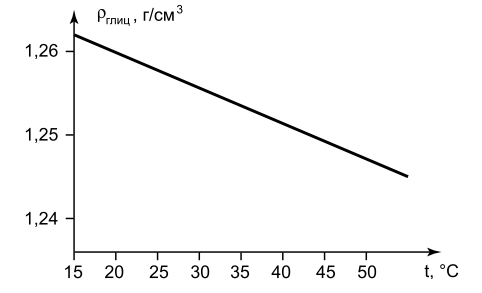
\includegraphics[height=5cm]{fluid2.png}
        \subcaption{Зависимость плотности глицерина от температуры}
    \end{subfigure}
\hfill
    \begin{subfigure}{0.45\textwidth}
        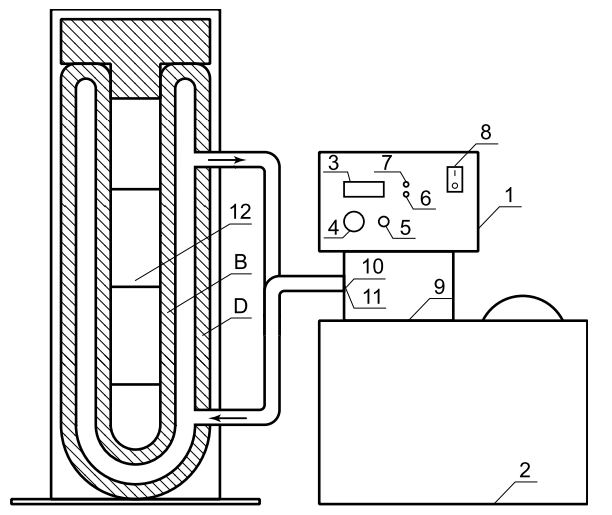
\includegraphics[height=5cm]{setup.png}
        \subcaption{Экспериментальная установка}
    \end{subfigure}
\end{figure}

% \section*{Экспериментальные данные}
%
%
% \begin{table}[h]!
%     \centering
%     \begin{tabular}{|c|c|c|c|c|c|c|c|c|c|c|c|c|c|c|c|}
%         \hline
%         № & 1 & 2 & 3 & 4 & 5 & 6 & 7 & 8 & 9 & 10 & 11 & 12 & 13 & 14 & 15\\\hline 
%         $d$, мм& & &
%         $\eta(T_1)$ &
%         $\eta(T_2)$ &
%         $\eta(T_3)$ &
%         $\eta(T_4)$ &
%         $\eta(T_5)$ & 
%     \end{tabular}
%     \caption{Зависимоть вязкости от температуры жидкости и диаметра шарика}
% \end{table}
%
% \begin{table}[h!]
%     \centering
%     \begin{tabular}{|c|c|c|c|c|c|}
%         \hline
%         $T^{\cdot}C$ & $T_1$ & $T_2$ & $T_3$ & $T_4$ & $T_5$\\\hline
%         $\rho_{\text{ж}}$, г/$\text{см}^3$ &  &  &  &  &
%     \end{tabular}
%     \caption{Зависимоть плотности жидкости от температуры}
% \end{table}
%
%
